%author : berenice delcroix-oger

\documentclass[border=2pt]{standalone}
\usepackage{tikz}
\usetikzlibrary{positioning, fit, shapes, arrows, calc}

\pgfdeclarelayer{bg}    % declare background layer
\pgfsetlayers{bg,main}  % set the order of the layers (main is the standard layer)

\newcommand{\coula}{0785F2}
\newcommand{\coulb}{F29F05}
\newcommand{\coulc}{F21313}
\newcommand{\could}{E6F21F}



\definecolor{part1}{HTML}{\coula}
\definecolor{part2}{HTML}{\coulb}
\definecolor{part3}{HTML}{\coulc}
\definecolor{part4}{HTML}{\could}

\begin{document}
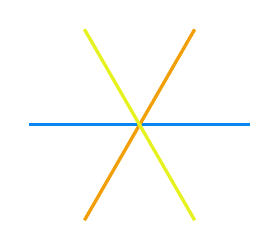
\begin{tikzpicture}[scale=0.7]
\coordinate (A) at (0:2);
\coordinate (B) at (60:2);
\coordinate (C) at (120:2);
\coordinate (D) at (180:2);
\coordinate (E) at (240:2);
\coordinate (F) at (300:2);
\draw[part1, very thick]  (A)--(D);
\draw[part2, very thick]  (B)--(E);
\draw[part4, very thick]  (C)--(F);
\end{tikzpicture}

\end{document}
